\section{Temporal Partitioning}

%%%%%%%%%%%%%%%%%%%%%%%%%%%%%%%%%%%%%%%%%

\begin{frame}{Real-Time Systems}

\pause
\begin{block}{Real-Time Constraints from Event to System Response}
\pause
\begin{itemize}[<+->]
    \item Deadlines based on real-time requirements
    \item No deadline misses allowed ever
    \item Prepare for the worst-case
\end{itemize}
\end{block}

\end{frame}


\begin{frame}{Real-Time Systems -- Scheduling Example}

\begin{block}{Task Set}
\begin{tabular}{cccc<{\onslide<3->}c<{\onslide}}
\textbf{Task}&\textbf{Period}&\textbf{Deadline}&\textbf{WCET}&\textbf{ACET}\\ \hline
$T1$&$10$&$5$&$4$&$2$\\
$T2$&$10$&$10$&$6$&$4$
\end{tabular}
\end{block}

\vfill

\includegraphics<2-3>[width=\textwidth]{Figures/real-time-sched-1}
\includegraphics<4>[width=\textwidth]{Figures/real-time-sched-2}

\end{frame}

\begin{frame}{Real-Time Systems -- Pros and Cons}

\begin{block}{}<2->
    \begin{itemize}
        \item<2-> Static guarantees even for the worst-case
        \item<3-> Overprovisioning for the average-case 
    \end{itemize}
\end{block}

\vfill

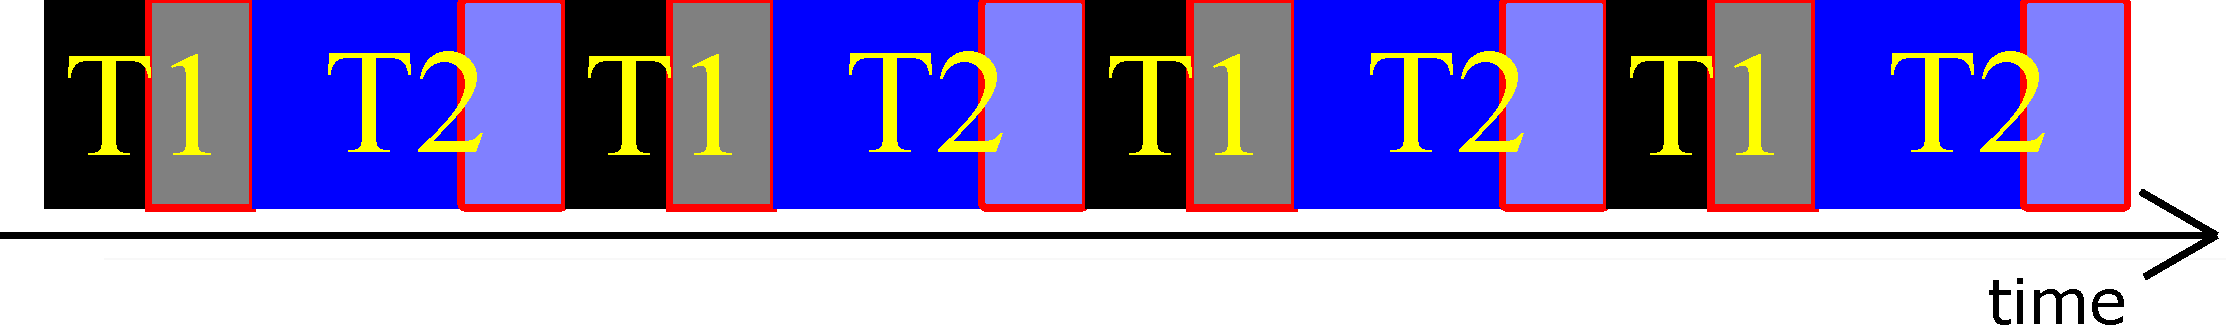
\includegraphics[width=\textwidth]{Figures/real-time-sched-2}

\onslide<4>{\centering \hilightA{Economic need for trading off guarantees for utilization}}

\end{frame}


%%%%%%%%%%%%%%%%%%%%%%%%%%%%%%%%%%%%%%%%%%%%%%%%%%%%%%%%%%%%%%%%%%%%%%%%%%%%%%
\subsection{Full-Scale Mode Switches}

\begin{frame}{Mixed Criticality Levels}

\begin{minipage}{\textwidth}
\begin{block}{Worst-Case Execution Time Estimates}<2->
\begin{itemize}
    \item<3-> Various components are validated against various assumptions
    \item<4-> The stricter assumptions, the longer estimated WCET
\end{itemize}
\end{block}

\vfill

\begin{block}{Criticality Levels of Tasks}<5->
\begin{itemize}
    \item<6-> Strictness of assumptions
    \item<7-> Ordered set of levels
\end{itemize}
\end{block}
\end{minipage}

\end{frame}

\begin{frame}{Mixed-Criticality Scheduling with Criticality Mode Switches}

\pause
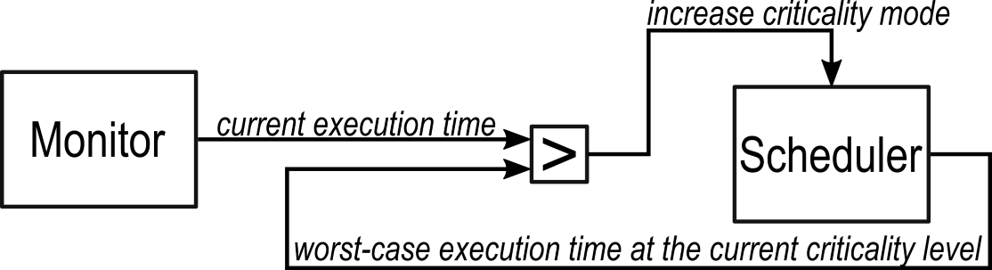
\includegraphics[width=\textwidth]{Figures/mixed-crit-sched-robin}
\pause
\begin{itemize}[<+->]
    \item Start system in the lowest criticality mode
    \item Schedule tasks with criticality not below the current criticality mode
    \item Monitor whether execution violates current assumptions
    \item Switch to higher criticality mode for stricter assumptions
\end{itemize}

\end{frame}


\begin{frame}{Mixed-Criticality Scheduling with Mode Switches}

\only<1-2>{%
\begin{minipage}{\textwidth}
\begin{block}{Task Set $HI$}
\begin{tabular}{cccc}
\textbf{Task}&\textbf{Period}&\textbf{Deadline}&\textbf{WCET}\\ \hline
$T1$&$10$&$5$&$4$\\
$T2$&$10$&$10$&$6$
\end{tabular}
\end{block}

\onslide<2>
\begin{block}{Task Set $LO$}
\begin{tabular}{cccc}
\textbf{Task}&\textbf{Period}&\textbf{Deadline}&\textbf{WCET}\\ \hline
$T1$&$10$&$5$&$2$\\
$T2$&$10$&$10$&$4$\\
$T3$&$10$&$9$&$3$
\end{tabular}
\end{block}
\end{minipage}
}

\only<3->{%
\begin{minipage}{\textwidth}
\begin{block}{Mixed-Criticality Task Set}
\begin{tabular}{ccccc}
\textbf{Task}&\textbf{CL}&\textbf{Period}&\textbf{Deadline}&\textbf{WCET}\\ \hline
$T1$&$HI$&$10$&$5$&$[2,4]$\\
$T2$&$HI$&$10$&$10$&$[4,6]$\\
$T3$&$LO$&$10$&$9$&$[3]$
\end{tabular}
\end{block}

\bigskip

\includegraphics<4>[width=\textwidth]{Figures/mixed-crit-sched-1}
\includegraphics<5>[width=\textwidth]{Figures/mixed-crit-sched-2}
\includegraphics<6>[width=\textwidth]{Figures/mixed-crit-sched-3}
\includegraphics<7>[width=\textwidth]{Figures/mixed-crit-sched-4}

\onslide<6->{\centering \hilightA{Ignoring $LO$ criticality tasks in $HI$ mode}}

\end{minipage}
}

\end{frame}

\begin{frame}{Limitations of Mode Switching Scheduling}

\pause
\begin{block}{Static Verification}\onslide<2->
\begin{itemize}
    \item<3-> Timing guarantees for each mode
    \item<4-> \hilightA{No link to requirements of safety standards}
\end{itemize}
\end{block}

\begin{block}{Runtime Robustness}\onslide<2->
\begin{itemize}
    \item<5-> Switching mode to restrict assumptions as necessary
    \item<6-> \hilightA{Ignoring low-criticality tasks}
    \item<7-> \hilightA{Returning to low-criticality mode}
\end{itemize}
\end{block}

\end{frame}


%%%%%%%%%%%%%%%%%%%%%%%%%%%%%%%%%%%%%%%%%%%%%%%%%%%%%%%%%%%%%%%%%%%%%%%%%%%%%%
\subsection{Memory Access Budgeting}

\begin{frame}{Memory Accesses and Execution Time}

\begin{block}{Cache Misses}<2->
\begin{itemize}
    \item<3-> Memory needs to be accessed
    \item<4-> Critical tasks may be penalized by interference
\end{itemize}
\end{block}

\begin{block}{Limited Interference for Critical Tasks}<5->
\begin{itemize}
    \item<6-> Reduce WCET of critical tasks by limiting interference
    \item<7-> Budget of cache misses for non-critical tasks (cores)
    \item<8-> Suspend execution of tasks with depleted budget
\end{itemize}
\end{block}

\vfill

\onslide<9->{\centering \hilightB{Can be generalized to any shared resource}}

\end{frame}

\begin{frame}{Memory Access Budgeting}

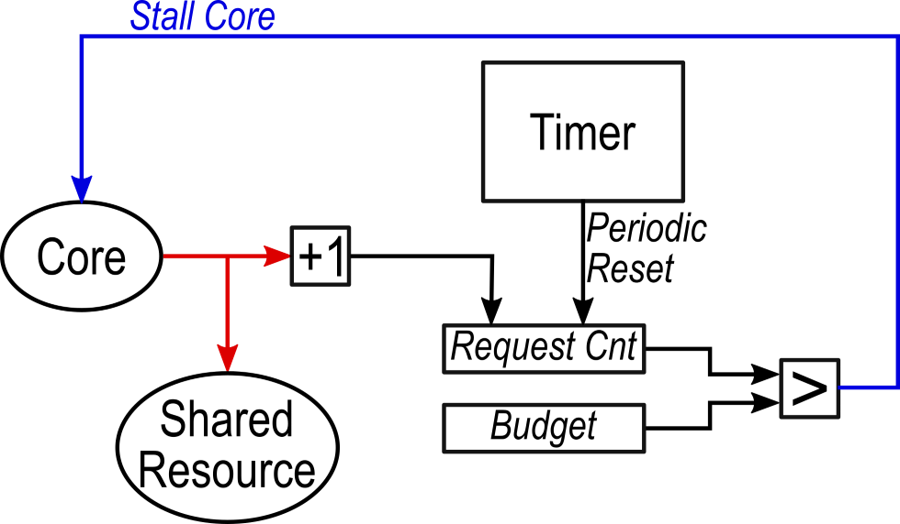
\includegraphics[width=\textwidth]{Figures/budgeting-robin}

\end{frame}


\begin{frame}{Memory Access Budgeting -- Pros and Cons}


\begin{block}{Pros}
\begin{itemize}
    \item<2-> Low overhead on COTS
    \begin{itemize}
        \item<3-> Performance counters
        \item<3-> Interprocessor interrupts
    \end{itemize}
\end{itemize}
\end{block}

\vfill

\begin{block}{Cons}
\begin{itemize}
    \item<4-> Limited to $2$ levels, critical and non-critical
    \item<5-> No general algorithm for deriving budgets
    \item<6-> Not scaling with the number of non-critical cores
\end{itemize}
\end{block}

\end{frame}

%%%%%%%%%%%%%%%%%%%%%%%%%%%%%%%%%%%%%%%%%%%%%%%%%%%%%%%%%%%%%%%%%%%%%%%%%%%%%%
\subsection{Execution Time Monitoring}

\begin{frame}{Monitoring Execution Time and Remaining WCET}

\begin{block}{WCET and Observation Points for Critical Tasks}<2->
\begin{itemize}
    \item<3-> Remaining WCET for each observation point
    \item<4-> Worst-case interference between observation points
\end{itemize}
\end{block}

\vfill

\begin{block}{Safety Condition at each Observation Point}<5->
The critical task will not miss its deadline even if worst-case happens until the next observation point
\end{block}

\end{frame}

\begin{frame}{Execution Time Monitoring}

Evaluate safety condition at each observation point:

\vfill

\begin{tabular}{lp{2pt}cl}
\onslide<2->{\color{olive}code segment $k-$}&&&\onslide<4->{\color{olive}execution time}\\
\onslide<3->{observation point $k$}&&&\\
\onslide<2->{\color{orange}code segment $k$}&&\onslide<4->{$+$}&\onslide<4->{\color{orange}$WCET_{interference}(k, k+1)$}\\
\onslide<3->{observation point $k+1$}&&&\\
\onslide<2->{\color{red}code segment $k+$}&&\onslide<4->{$+$}&\onslide<4->{\color{red}$WCET_{isolation}(k+1, end)$}\\
&&&\\
&&\onslide<4->{$+$}&\onslide<4->{\color{purple}observation overhead}\\
&&&\\
&&\onslide<4->{$<$}&\onslide<4->{deadline}
\end{tabular}

\vfill

\onslide<5->{%
Suspend non-critical tasks if safety condition does not hold.
}

\end{frame}


\begin{frame}{Execution Time Monitoring -- Pros and Cons}

\begin{block}{Pros}
\begin{itemize}
    \item<2-> Code instrumentation is easy to implement on COTS
    \item<3-> Monitoring execution time limits pessimism
    \item<4-> Evaluating condition at observation points limits pessimism
\end{itemize}
\end{block}

\vfill

\begin{block}{Cons}
\begin{itemize}
    \item<5-> Limited to $2$ levels, critical and non-critical
    \item<6-> Large execution time overhead of monitoring
\end{itemize}
\end{block}

\end{frame}


%%%%%%%%%%%%%%%%%%%%%%%%%%%%%%%%%%%%%%%%%%%%%%%%%%%%%%%%%%%%%%%%%%%%%%%%%%%%%%
\subsection{Workload Arrival Monitoring}

\begin{frame}{Workload Arrival Monitoring}

\begin{block}{Workload Arrival Function (WAF) for each Task}<2->
\begin{itemize}
    \item<3-> Task is activated by events
    \item<4-> The events are mapped to WCET values
    \item<5-> WAF accumulates required execution time
\end{itemize}
\end{block}

\begin{block}{Arrival Monitoring and Admission}<6->
\begin{itemize}
    \item<7-> Actual workload is calculated based on WAFs
    \item<8-> Check whether workload would exceed serviceable level
\end{itemize}
\end{block}

\onslide<9->{\centering \hilightB{Individual WAFs enforce interference bounds between real-time tasks}}

\end{frame}

\begin{frame}{Group Monitoring Scheme}

\begin{block}{Criticality Groups}<2->
\begin{itemize}
    \item<3-> Tasks of one criticality level are grouped together
    \item<4-> A group of tasks is one virtual task for workload arrival
    \item<5-> Correlation of task activations improves utilization
\end{itemize}
\end{block}

\begin{block}{Combining Monitors}<6->
\begin{itemize}
    \item<7-> Monitors for groups separately
    \item<8-> Each monitor respects WAF upper bounds
    \item<9-> Monitors are synchronized by guarantee interface tuples
    \item<10-> Pareto interface tuples with maximized individual WAFs
\end{itemize}
\end{block}

\end{frame}


\begin{frame}{Workload Arrival Monitoring -- Pros and Cons}

\begin{block}{Properties}<2->
\begin{itemize}
    \item<3-> \hilightB{Event-triggered}
    \item<4-> \hilightA{Considering worst-case is highly pessimistic}
    \item<5-> \hilightB{Group monitoring provides more accurate assumptions}
\end{itemize}
\end{block}

\end{frame}

%%% Local Variables:
%%% mode: latex
%%% TeX-master: "slides"
%%% End:
